%!TEX root = main.tex

\begin{figure*}[t!]
\centering
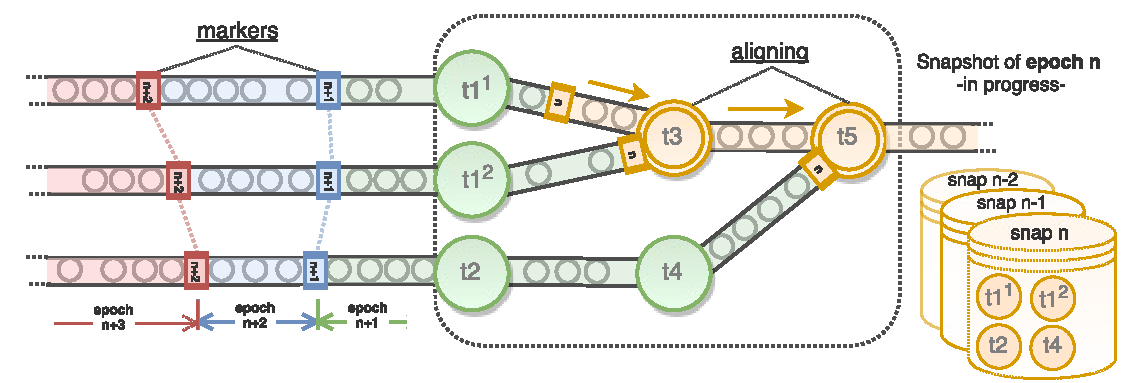
\includegraphics[width=\textwidth]{figures/snapshots-overview.pdf}
\caption{An Example of the Pipelined Snapshotting Protocol.} 
\label{fig:snapshots-overview}
\vspace{-4mm}
\end{figure*}

\section{Core Concepts and Mechanisms}
\label{sec:core}

\subsection{System Model}

Each processing pipeline in Flink translates into a logical directed graph $G = (\mathcal{T}, \mathcal{E})$ consisting of a set of vertices $\mathcal{T}$ representing tasks of finest-grained computation and a set of edges $\mathcal{E}$ reprenting data channels between tasks in $\mathcal{T}$. A task $t \in \mathcal{T}$ can encapsulate the logic of a single user-defined operation (e.g., \texttt{map}, \texttt{filter}, \texttt{fold}) or multiple operations that are fused together. Fusion is a standard logical dataflow optimisation \cite{hirzel2014catalog,chambers2010flumejava} which is also applied on Flink during the composition of $G$. 

\subsubsection{Managed State}

Each stream operation in Flink can declare consistent state and update it continuously in order to keep a summary of the data seen so far. State is a main building block of a pipeline since it encapsulates, at any time the full status of the computation. There are conceptually two scopes upon which managed state operates. For purely data-parallel stream operations such as for example a per-key average, state and associated streams are logically scoped and operate independently for every key. We refer to this state as \texttt{Keyed-State}. For local, per-task computation such as for example a partial machine learning training model, state can be declared in the level of a physical dataflow task, known as \texttt{Operator-State}. Both \texttt{Keyed-State} and \texttt{Operator-State} respectively are transparently partitioned and managed by the runtime of the system. More importantly, the system can guarantee that update operations on managed state will be invoked exactly-once with respect to the input streams. In section \ref{sec:implementation} we explain in detail how the file system facilitates efficient out-of-core state persistence of different state types despite the local  view exposed to the programmer. Below, we briefly explain how managed state can be declared and the basic intuition for each of the state types. \paris{@stefan : Please check and elaborate more in this subsection}

\para{\texttt{Keyed-State}}: Any stream computation can be mapped to a user-defined key space and as a result any associated state will also scoped together with the computation. Typically, data stream records arrive to the system with some domain-specific key such as a user-session identifier, a device address or a geographical location. In the most general case, Flink allows for a user to map any record from its schema domain $\mathcal{S}$ to a given key space $\mathcal{K}$ via the $\texttt{keyby}: \mathcal{S} \rightarrow \mathcal{K}$ operation supported by the \texttt{DataStream} abstract type. Under key scope, state can be allocated dynamically within a user-defined function by using special collections that the model exposes through the API and vary depending on the nature of the state. For append-only state per key (e.g. for storing a pattern sequence or a window) there is a \texttt{ListState} collection supporting an \texttt{add} operation. If  the state is otherwise a value that mutates during the application logic, there is a \texttt{ValueState} type supporting an \texttt{update} operation. Other basic state types such as \texttt{ReduceState} also allow for one or two-step, on-the-fly, distributive function aggregations on managed state. 

\para{\texttt{Operator-State}}: When a DataStream is not scoped by key, state and processing operate per parallel physical instance of a task. This is typical when computation is for example relevant to each physical stream partition such as the source instances of a pipeline that correspond to Kafka consumers in a 1-1 mapping of active offset per partition. Operator-state types are similar to Keyed-State (i.e., \texttt{ListState}, \texttt{ValueState}). 

\subsubsection{State Partitioning and Allocation}

The mapping of a logical dataflow graph to $G$, the physical, distributed execution graph occurs when a pipeline is deployed, on its initial run or upon reconfiguration (e.g., for scale-out). During that stage each logical task $t \in \mathcal{T}$ is mapped to a number of physical tasks $t^1, t^2, \ldots, t^\pi$, each of which gets allocated to available containers throughout a cluster (e.g., using YARN \cite{vavilapalli2013apache}) up to the decided degree of parallelism $\pi \in \mathbb{N^+}$. For tasks that have declared managed state, it is important to consistently allocate data stream partitions or re-allocate in the case of reconfiguration. The partitioning process makes sure that each parallel physical task $t^i , \forall i : 0 \leq i \leq \pi$ will only receive records (and maintain state) that belong to a pre-allocated range of keys. Since the key space $\mathcal{K}$ can be user-defined Flink's runtime pre-partitions keys to an intermediate circular space of ``key-groups'' : $K^* \subset \mathbb{N^+}$ given a maximum parallelism $\pi\text{-max}$ and a hash function $h$ as such:

\noindent $K^* = \{ h(k)\text{ \texttt{mod} }\pi\text{-max}\text{ }|\text{ }k \in \mathcal{K}, \pi\text{-max} \in \mathbb{N^+}, h: \mathcal{K} \rightarrow \mathbb{N^+} \}$

Upon deployment with parallelism $\pi$ key groups are directly allocated per task $t^i$ from $\lceil i \times \frac{\pi\text{-max}}{\pi} \rceil$ to $\lfloor (i+1) \times \frac{\pi\text{-max}}{\pi} \rfloor$. We found that this is a trivial way to pre-partition and reallocate state in a pipeline, typically using a non-cryptographic hash function such as murmur hash. As shown in \autoref{sec:implementation}, state snapshots are materialized and indexed per allocated key group at the backend which allows for trivial reconfiguration. \paris{@stefan I need some input regarding operator state rescaling.}

\subsection{The Pipelined Snapshotting Protocol}
\label{sec:snapshots}
Flink's snapshotting protocol provides a uniform way to capture the complete state of a pipeline and roll it back whenever that is required. We will first explain its intuition followed by a more formal definition of the assumptions and description of the protocol for directed acyclic and cyclic graphs respectively.

\subsubsection{Approach Intuition}

A continuous stream execution is conceptually divided into logical periods that ``cut'' a distributed data stream into consecutive finite sets of records \ref{fig:abs-general}, which we call \emph{epochs}. An \emph{epoch} can be triggered on-the-fly, periodically by the system or on-demand by the user and is decoupled from any application logic (e.g., windowing constrains). A snapshot of the computation at \emph{epoch} $n$ refers to a copy of the internal state of each task $t \in \mathcal{T}$ after the system fully ingests every input record from the beginning of the computation (\emph{epoch} 0) up to and including \emph{epoch} $n$. In case of a failure during or before a snapshot of \emph{epoch} $n$ is acquired we can simply revert the global state of the distributed dataflow graph to a previous \emph{epoch} (e.g., $n-1$). A discrete approach to snapshotting would be to let the distributed dataflow fully ingest \emph{epoch} $n$ independently, store the internal state of each task $t \in \mathcal{T}$ and proceed with \emph{epoch} $n+1$ (similarly to micro-batching \cite{zaharia2012discretized}). However, this approach generally leads to high latency and underutilization costs related to the coordination of a discrete execution which cannot be amortized trivially \cite{venkataramandrizzle}. Furthermore, other protocols either disrupt normal execution \cite{murray2013naiad,jacques2016consistent} or are incapable of supporting weakly connected graphs \cite{chandy1985distributed} which are the norm in distributed dataflow processing.

Instead, Flink's snapshotting protocol pipelines progressively the partial acquisition of task states to eventually acquire a complete snapshot, respecting \emph{epochs}, while running concurrently alongside normal operation. Special markers are injected in each data stream partition at the dataflow sources, coordinated by the runtime and get disseminated throughout the dataflow graph as depicted in \autoref{fig:snapshots-overview}. Markers signal distributed tasks of new epochs and thus aid to establish the appropriate moment to snapshot each local state and proceed with further processing promptly. Tasks with multiple inputs execute an \emph{alignment} phase (e.g., tasks $t3$ and $t5$ in \autoref{fig:snapshots-overview}) upon which they prioritize inputs from pending \emph{epochs}. Alignment is decentralized and eliminates the need to forcefully consume an epoch or log records in transit in the case of acyclic graphs. As we explain in more detail further, cyclic graphs require partial channel logging only limited to each dataflow cycle. The snapshotting protocol is coordinated centrally by the \emph{JobManager} and each invocation eventually completes or gets aborted (e.g., when a failure occurs). In either case the overall dataflow computation can always progress without interruptions and consecutive snapshots will eventually complete.

\subsubsection{Main Assumptions}

The protocol assumes a fail-recovery, deterministic process model \cite{elnozahy2002survey} where a partial process failure can be masked by redeployment and restoration of prior operational states. In detail, our protocol builds on the following assumptions:

\begin{itemize}
	\item Input data streams are durably logged and indexed by an external logging system such as Apache Kafka \cite{kreps2011kafka}. That means that dataflow sources can trivially re-consume input from a specific logical time by requesting an offset per stream partition. 
	\item Directional data channels between tasks are quasi-reliable, respect a FIFO delivery order and can be blocked or unblocked. When a channel is blocked in-transit messages are internally buffered (and possibly spilled to disk) and can be delivered on that end once it unblocks.
	\item Tasks can trigger a \texttt{block} or \texttt{unblock} operation on their input data channels and \texttt{send} events (records or control messages) through their output channels.
\end{itemize}

\subsubsection{Directed Acyclic Graphs}

\begin{algorithm}
$inputs$ $\leftarrow$ configured\_inputs\;
$outputs$ $\leftarrow$ configured\_outputs\;
$blocked \leftarrow \emptyset$ \;
% $operator$ $\leftarrow$ dataflow\_operator\;

\Hdl{$\langle marker \rangle$ from $in \in inputs$}{
\If{$in \neq Nil$}{
 $blocked \leftarrow blocked \cup in$\;
 $in$.block()\;
}
\If{$blocked = inputs$}{
\ForEach{$out \in outputs$}{
$out$.send($\langle marker \rangle$)\;
}
triggerSnapshot()\;
\ForEach {$in \in inputs$}{
$in$.unblock()\;
}
$blocked \leftarrow \emptyset$ \;
}
}
\caption{Snapshot Alignment}
\label{alg:snapdag}
\end{algorithm}

\begin{figure}[t]
\centering
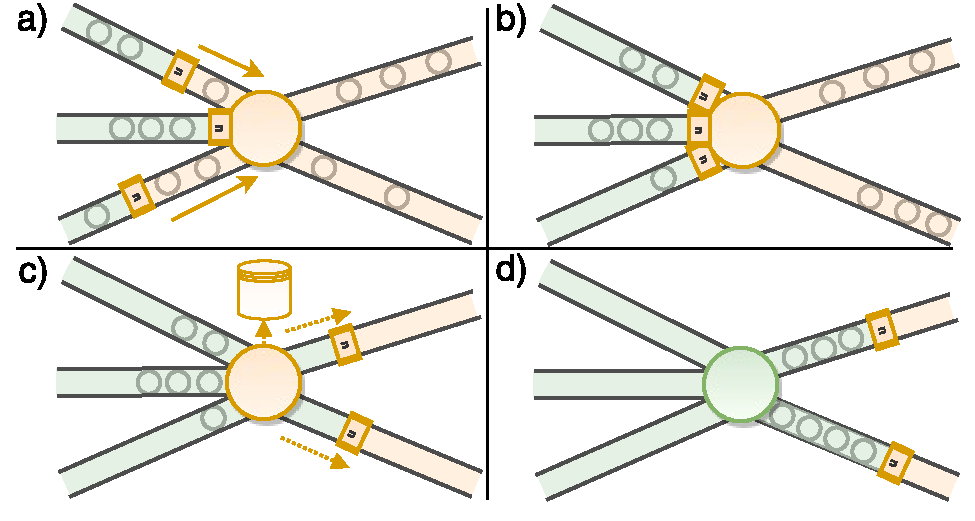
\includegraphics[width=\textwidth / 2]{figures/snapshots-highlights.pdf}
\caption{Alignment and Snapshotting Highlights.} 
\label{fig:snapshots-highlights}
\vspace{-4mm}
\end{figure}

Let us consider only directed acyclic graphs (DAGs) for now. The protocol gets initiated at the source tasks of the dataflow by the \texttt{TaskManager}, however, for simplicity we assume here that the logic gets initiated upon receiving a special marker event in each and every task (sources would ``receive'' that first through a $Nil$ channel). \autoref{alg:snapdag} summarizes the snapshot alignment and pipelining protocol that executes when a marker is received. Mind that this runs in the same low level, record handling thread that also invokes user-defined operators (i.e., records and markers are handled sequentially by the same thread). 

\para{Alignment:} \autoref{fig:snapshots-highlights} vizualizes the steps prior to and during snapshotting in more detail. When a task receives a snapshot marker on one of its inputs it blocks that channel since all computation associated with the current epoch has to finish before continuing further (\autoref{fig:snapshots-highlights}(a)). The blocking operation might result into spilling of in-transit records within that channel to disk, if allocated memory for network buffers reaches its limit. Once markers have been received in all inputs (\autoref{fig:snapshots-highlights}(b)) the task can proceed with snapshotting while also notifying downstream tasks. In the same atomic operation markers are broadcasted further and local snapshotting is triggered concurrently(\autoref{fig:snapshots-highlights}(c)). Depending on the backend support, snapshots can be triggered and be executed asynchronously by another thread, thus, inducing zero impact to the overall throughput. Once local snapshotting is initiated all input channels are unblocked and the computation continues as normal (\autoref{fig:snapshots-highlights}(d)) in the next epoch.

\subsubsection{Dealing with Dataflow Cycles}

\begin{algorithm}
$outputs$ $\leftarrow$ configured\_outputs\;
$isLogging \leftarrow false$ \;
$log \leftarrow \emptyset$ \;

\Hdl{$\langle marker \rangle$}{
\eIf{$isLogging$}{
triggerSnapshot($log$) \;
$log \leftarrow \emptyset$ \;
}{
$isLogging \leftarrow true$ \;
\ForEach{$out \in outputs$}{
$out$.send($\langle marker \rangle$)\;
}
}
}
\Hdl{$record$}{
\If{$isLogging$}{
 $log \leftarrow log \cup record$\;
}
\ForEach{$out \in outputs$}{
$out$.send($record$)\;
}
}
\caption{Snapshotting in Cycles}
\label{alg:snapcycle}
\end{algorithm}


Dataflow graphs in Flink can also support cycles. Cycles are currently defined explicitly through Flink's programming API as asynchronous iterations, though structured iterations (e.g., on stream windows) are also considered and can be supported in the future. Snapshotting within cycles in dataflow graphs are being handled as a special case and implemented by specific tasks which we call Iteration Sources. Each dataflow cycle is orchestrated through two implicit tasks: an \texttt{IterationHead} and \texttt{IterationTail}. These two tasks types give the impression of regular dataflow \emph{source} and \emph{sink} respectively, however, they are collocated to share an in-memory buffer and thus implement the feedback logic (and cyclic snapshotting) without being exposed to the developer.

\begin{figure}[t]
\centering
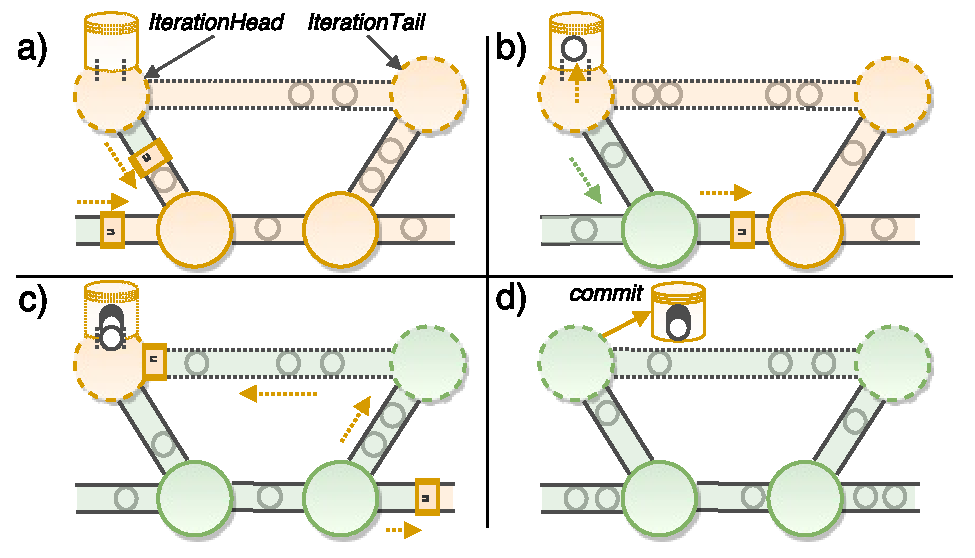
\includegraphics[width=\textwidth / 2]{figures/cycle-highlights.pdf}
\caption{Cycle Snapshotting Highlights.} 
\label{fig:cycle-highlights}
\vspace{-4mm}
\end{figure}

The default stream alignment logic presented (\autoref{alg:snapdag}) would result into an incomplete distributed snapshot if it would be applied \emph{apriori} on cyclic graphs. That is due to the fact that records belonging to prior epochs could still remain indefinitely in-transit within a cycle even after a snapshot has been taken over. Thus, it is of high importance to include these records in the snapshot (or their side effects) in order to get a complete picture of the correct distributed execution \cite{chandy1985distributed,elnozahy2002survey}. Alternative approaches to this problem consider a ``flushing'' phase which enforces the inclusion of all the in-transit records to the internal state of each operator \cite{jacques2016consistent}, however, we argue that this is only relevant to the state of a cycle. Thus, we execute a similar special logging protocol that runs transparently and solely within the \texttt{IterationHead} instances of each cycle.

As described in detail in \autoref{alg:snapcycle} and also visualized in \autoref{fig:cycle-highlights}, \texttt{IterationHead} tasks receive a special marker from the runtime signifying each epoch, same as the sources of the dataflow graph. At that instance, they disseminate markers further within a cycle and start logging in their own registered managed state all in-transit events that exist within a cycle in that respective partition (\autoref{fig:cycle-highlights}(a)). Once the marker of the snapshot is received back through their respective collocated \texttt{IterationTail} (\autoref{fig:cycle-highlights}(c)) they trigger a snapshot of that log containing a complete upstream log of all records in-transit that belong to that epoch (\autoref{fig:cycle-highlights}(d)). It is important to note that the default alignment protocol that runs in the rest of the tasks within a cycle (\autoref{fig:cycle-highlights}(b)) ensures that no records belonging to subsequent epochs will transit prior to the marker and thus the complete state of a cycle is logged consistently. This special logic also restricts channel logging to cycles and does not enforce anything other than task states to be included in the snapshot for the rest of the dataflow graph (unlike Chandy and Lamport's \cite{chandy1985distributed} algorithm or state-of-the-art protocols that focus on weakly connected dataflow graphs \cite{elnozahy2002survey,jacques2016consistent,murray2013naiad}).


\subsection{Savepoints and Consistent Rollback}

Distributed snapshots, described previously in \autoref{sec:snapshots} form the basis for a variety of operations using the Apache Flink system. A snapshot contains all fundamental metadata required to retrieve the complete pipeline state from an associated durable storage backend such as references and indexes to task state partitions and upstream logs (in case of cyclic graphs). Periodic snapshots are automatically triggered by Flink's runtime as a form of per-job ``checkpoint'' for the purposes of consistent fail recovery whenever partial failures occur. However, the usages of snapshots go beyond fault tolerance needs. For a system that is widely deployed in a cloud infrastructure, having the ability to trivially scale resources in or out and lease containers is nowadays a necessity. In principle, failover and re-scaling are two operations that share the same underlying need of adaptive and consistent reconfiguration support \cite{castro2013integrating}. In this section we describe in more detail the operational benefits that distributed snapshots make feasible, as well as the rollback reconfiguration schemes that are currently supported.

\subsubsection{Savepoints and Usages}
Flink's snapshots offer a lightweight, yet complete ``materialized view'' of a continuous pipeline which can be used in arbitrary ways to load, re-partition and therefore re-deploy otherwise complicated states right out from distributed storage. Snapshots are, in fact, also exposed to the user or operations engineer in the manageable and flexible form of \emph{savepoints}. A \emph{savepoint} is an externally stored snapshot (i.e., the metadata pointing to pipeline state) that can be managed by users for various custom operational needs. For example, when a new version of the system is released it is recommended to trigger a savepoint for each active pipeline, upgrade the system, and then restore all pending computations at the epoch that they were left of. Other common usages of savepoints are to update application logic (e.g., software patches) of already running jobs by replacing operators accessing the same snapshotted state or adding new state entries instead. In turn, the ability to restore computation and repartition state on updated application logic further enables forking and versioning capabilities, similarly to version control systems, yet in a distributed continuous processing environment. Finally, Flink also allows periodic snapshots to be externalized in the form of savepoints on configured directories for cases where an operations expert, for example, prefers to do manual bookeeping of pipeline states and perhaps keep a logged history of the overall computation. \paris{perhaps we could elaborate more here and add a motivating figure with snapshots and usages}

\subsubsection{Consistent State Rollback}

\paris{Recovery is probably the weakest part of state management. We restart the whole thing whenever we have to reconfigure and this is honestly a bit bad but hey it's simple. (also spark does this for every microbatch so maybe it is not that sad)}



